\documentclass[xetex,mathserif,serif]{beamer}

\usepackage{beamerthemesplit}
\usetheme{Rochester}
\usecolortheme{lily}

\usepackage{minted}
\setminted{autogobble, mathescape}
\usemintedstyle{tango}

\title{Pragmatic \LaTeX}
\author{Nicholas Lantz}
\date{October 20, 2016}

\begin{document}
\maketitle

\begin{frame}
    \frametitle{What is \LaTeX?}

    \begin{itemize}
        \item
            A typesetting and document preparation system
        \item
            Looks better than Word
        \item
            Written especially for writing technical reports
    \end{itemize}
\end{frame}

\begin{frame}
    \frametitle{Ligatures}
    \framesubtitle{\LaTeX Vs. Word}

    \begin{itemize}
        \item
            Certain character combinations look awkward together, for
            example\ldots
    \end{itemize}

    \Large
    find vs. {f}ind\\
    fly vs. {f}ly\\
    efficient vs. e{f}{f}{i}ccient
\end{frame}

\begin{frame}
    \frametitle{Typesetting Math}
    \framesubtitle{\LaTeX Vs. Word}

    \begin{itemize}
        \item
            We go to Mines, we all need to typeset mathematical equations for
            projects, lab reports, etc.
        \item
            \LaTeX supports these very nicely, and the output looks much better
            than the Word equivalent.
    \end{itemize}

    \centering
    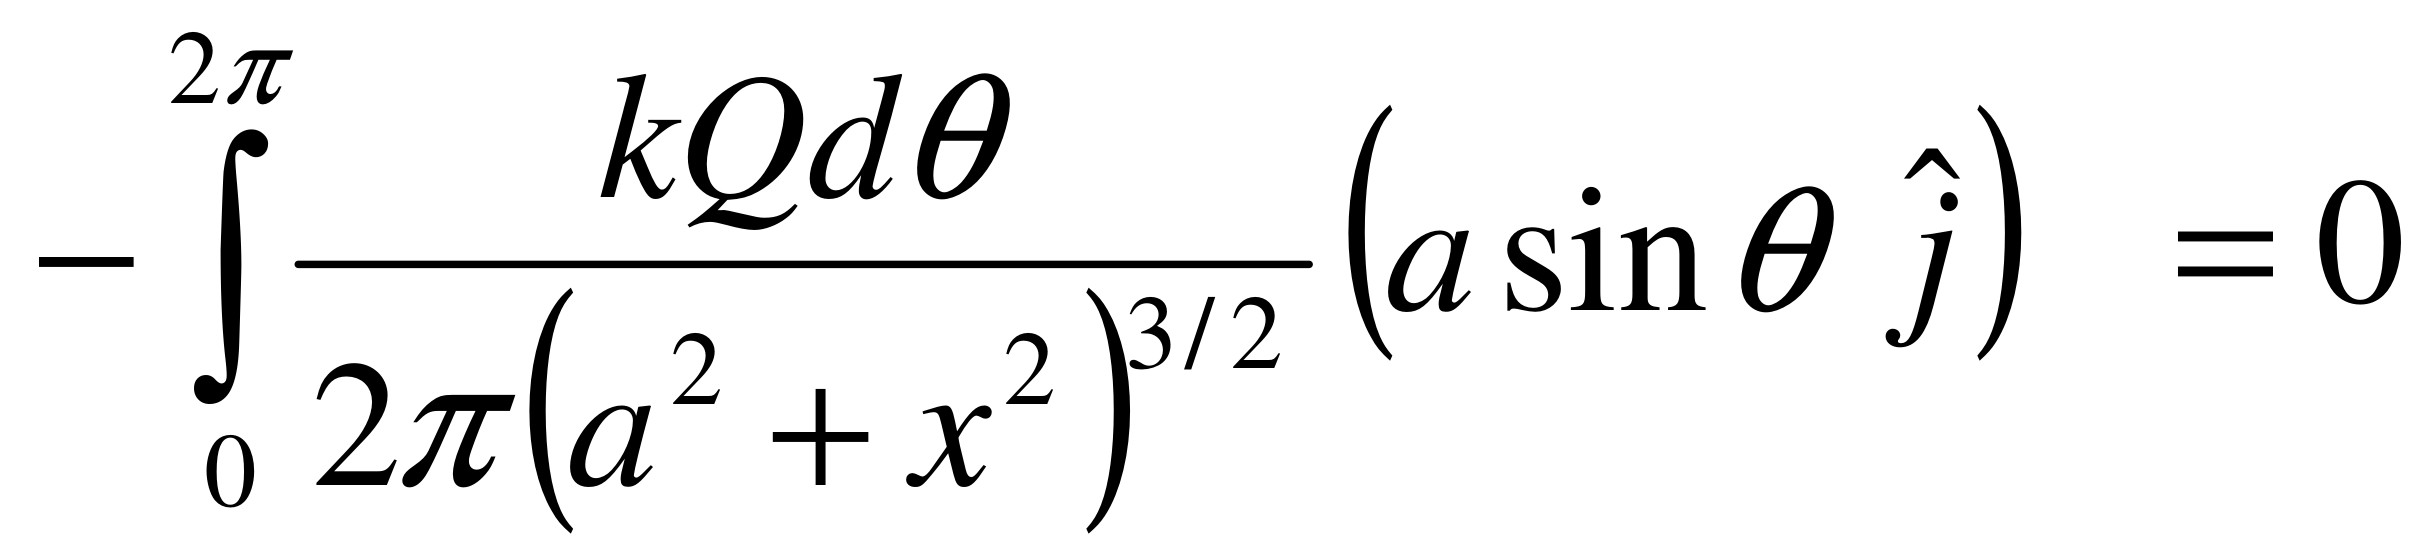
\includegraphics[width=2.5in]{media/wordmath}

    \begin{displaymath}
        -\int_0^{2 \pi} \frac{kQ\, d\theta}{2\pi{\left(a^2 +
        x^2\right)}^{3/2}} (a \sin \theta \,\hat\jmath) = 0
    \end{displaymath}
\end{frame}


\end{document}
